\mysection{Experimental setup}\label{sec:setup}
%We demonstrate linear feedback cooling of two translational modes simultaneously. 
The experiment consists of a permanent magnet levitating in a superconducting trap by Meissner repulsion. The motion of the magnet is measured using a Superconducting QUantum Interference Device (SQUID) measured by a lock-in amplifier. The lock-in then calculates a feedback signal and sends this to a piezoelectric actuator, schematically shown in Fig.~\ref{fig:setup}a.

%A piezoelectric actuator is used to cool translational modes by means of linear feedback. 

%The experiment is performed at the bottom of an extensive vibration isolation system inside a dry dilution refrigerator, and is schematically shown in Fig.~\ref{fig:setup}a. Cooling to the quantum ground state with the same technique is possible, with additional vibration isolation particularly for the lower frequencies (resonances of the vibration isolation system), and improved detection coupling with the use of a quantum limited SQUID.

The permanent levitating magnet is composed of three \SI{0.25}{mm} by \SI{0.25}{mm} by \SI{0.25}{mm} cubic neodymium iron boron parylene coated magnets stacked and glued together, using Stycast. A glass sphere with a diameter of \SI{0.20}{mm} is attached to this stack of magnets, again using Stycast, see Fig.~\ref{fig:setup}b. The glass sphere is placed off center to break symmetry. Typical permanent remnant magnetisation of these magnets is \SI{1.4}{T}, although it is believed that at low temperatures this is reduced by \SIrange{20}{25}{\%}~\cite{NdFeB_SmCo_Technotes}. The estimated mass of this composed magnet and glass sphere is \SI{0.35}{mg}.

The magnet levitates in a type I superconducting trap made of tantalum, shown in Fig.~\ref{fig:setup}c. This trap has an elliptical shape, \SI{3.0}{mm} by \SI{4.0}{mm} as the minor and major axes. The pick-up coil is placed at a height of \SI{4.0}{mm} from the bottom of the trap. The calculated levitation height of the magnet is \SI{1.96}{mm}~\cite{Vinante2020}. The pick-up coil is able to detect the motion of the magnet, via the induced current in the pick-up coil. The pick-up coil is part of the detection scheme consisting of the pick-up coil, the calibration transformer, and the SQUID input coil. The calibration transformer is used to calibrate the coupling between the detection circuit and the six different degrees of motion of the magnet. A schematic overview of the detection can be seen in Fig.~\ref{fig:setup}a.
%levitation height: https://www.wolframalpha.com/input?i=%28%283*mu_0*%283*0.25mm*0.25mm*0.25mm*1.4T%2Fmu_0%29%5E2+%29+%2F+%2864*pi*0.354e-6+kg*9.81m%2Fs%5E2%29%29%5E%281%2F4%29

\begin{figure}[t!]
    \centering
    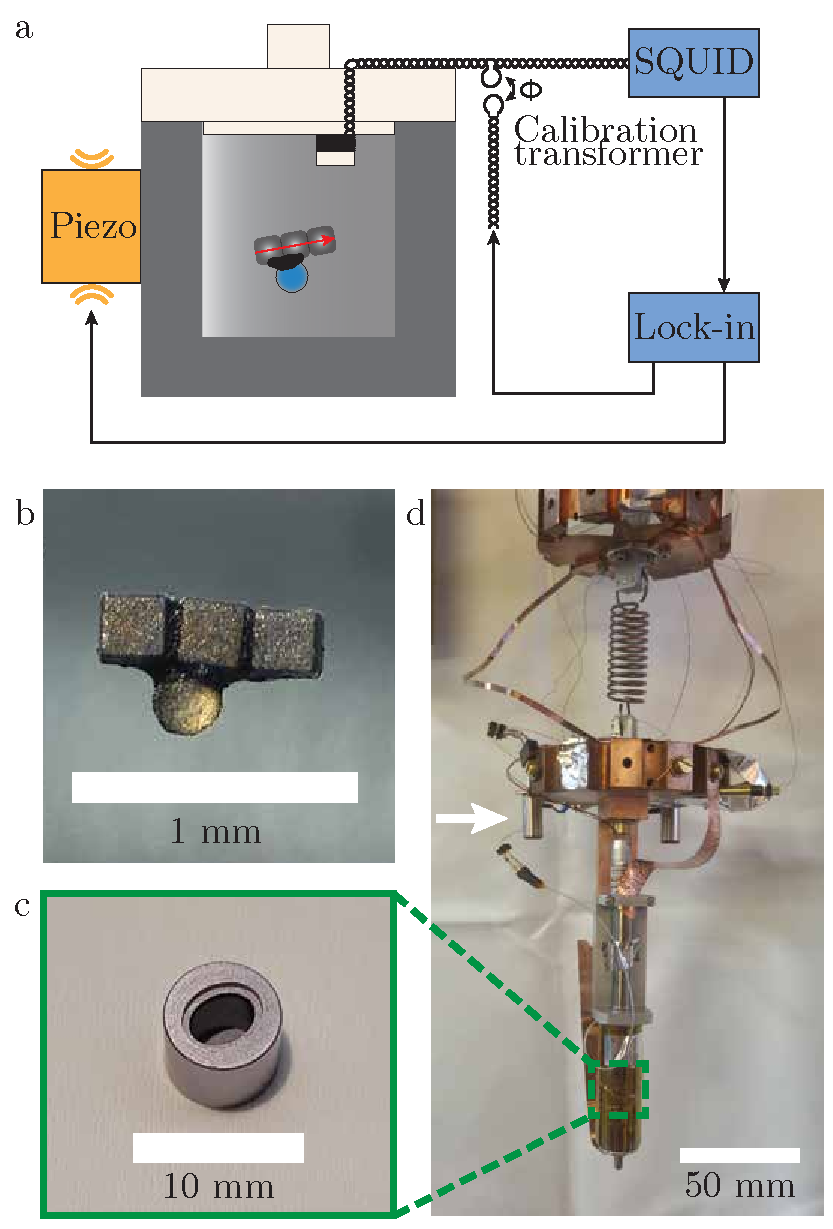
\includegraphics[width=\columnwidth]{Figures/Figure_setup_new_V2.pdf}
    \caption{Overview of the experimental setup. (a) A schematic outline of the setup, the levitating permanent magnet is shown inside the superconducting trap. A pick-up coil attached to the lid of the trap picks up the varying flux of the moving levitated magnet and is detected using a two stage SQUID amplifier. We feedback cool the magnets motion by applying a phase shifted tone shaking the trap housing through a piezo and lock-in amplifier. (b) A close-up of the permanent magnet used in the experiment. It is composed of three \SI{0.25}{mm} cubic neodymium iron boron parylene coated magnets stacked and glued together. A glass sphere with a diameter of \SI{0.20}{mm} is attached to this stack of magnets using Stycast, to break rotational symmetries. (c) Picture of the elliptically shaped superconducting trap, made from tantalum. (d) Closeup of the bottom part of the multi-stage mass spring system where the magnet, trap and piezo are located. The trap is located inside the magnetic shielding, indicated with the green dashed lines. The piezo is attached to the lowest copper mass and indicated with a white arrow.}
    \label{fig:setup}
\end{figure}

Vibrational noise is suppressed by a multistage mass spring system both in the vertical and lateral directions. The lowest two masses and one of the springs can be seen in Fig.~\ref{fig:setup}d. The experiment is rigidly attached to a copper mass, which is suspended from two other copper masses with springs in between. The lowest resonance frequencies are at \SI{0.6}{Hz} and \SI{1}{Hz} along the lateral and vertical directions, respectively. These three stages are thermalised to the millikelvin stage inside a dry dilution 

%\DU{De opmaak hier is vrij lastig, moet helaas met de hand}
\clearpage
\begin{widetext}
\begin{figure}[t]
    %\centering
    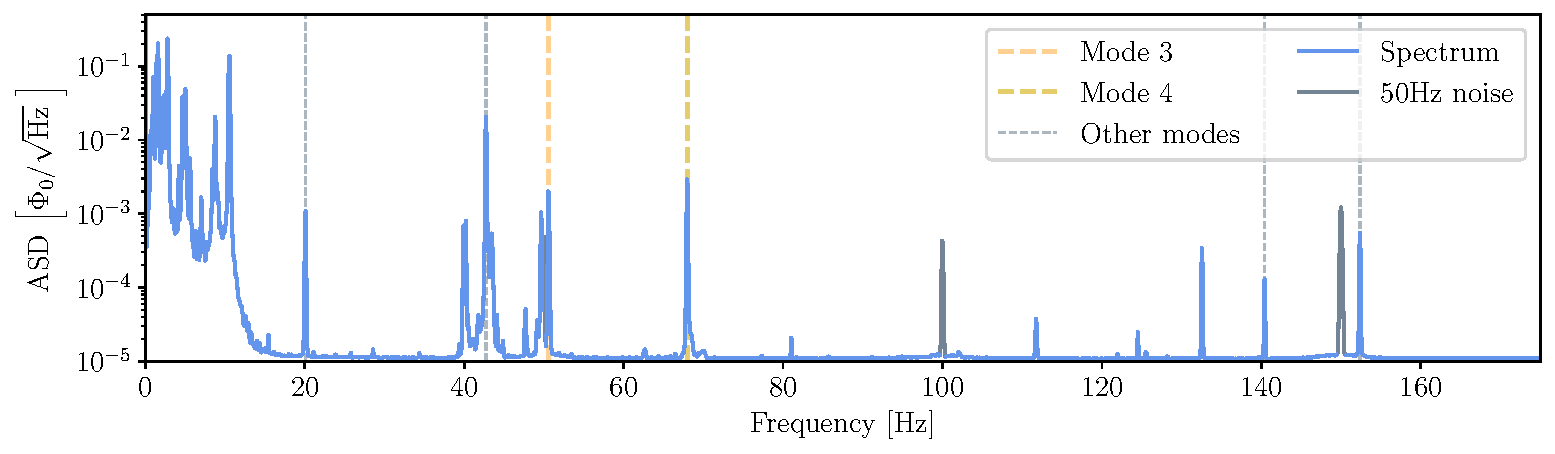
\includegraphics[width=\textwidth]{Figures/paper_figure_spectrum_20260307_during_the_day.pdf}
    \begin{minipage}{\textwidth}
    \caption{Typical amplitude spectral density (ASD) of the levitated magnet, the resonant modes of the magnet are indicated with the dotted lines. In this figure the \SI{50}{Hz} European electrical noise is grayed out.}
    \label{fig:spectrum} \end{minipage}
\end{figure}
\end{widetext}

\noindent
refrigerator. In the current configuration, the mass spring system is suspended from the still plate in order to utilize the additional available vertical length. For further attenuation, the still plate is suspended by springs from the \SI{3}{K} plate. 

The cryostat as a whole is rigidly attached to a 25-metric ton concrete block located in the cellar of the building, placed on pneumatic dampers to limit vibrations. The pulse tube and circulation pumps are rigidly attached to the building via a second frame. We typically measure between \SI{110}{} and \SI{130}{dB} attenuation in energy at a frequency range of \SIrange{50}{70}{Hz}, for this system. This is consistent with a finite element simulation, which show between \SI{160}{} to \SI{180}{dB} under idealized conditions, see supplementary material Fig.~\ref{fig:spectrum_attenuation}. 

%\red{We typically measure 80 dB attenuation in a frequency range of \SIrange{15}{80}{Hz}, for this system.\red{eventueel nog iets zeggen (apart) over 80-180Hz)} This is in agreement with a finite element model.}  
%The experiment is rigidly attached to a copper mass, which is hanging from two other copper masses, with a \textcolor{cyan}{lowest resonance frequency at \SI{10.67}{Hz}.} \DU{@Jurriaan?} These three stages are all thermalised to the millikelvin stage inside the dry dilution refrigerator. The mass spring system, however, is hanging from the still plate to use the extra length. For further attenuation, the still plate is suspended by springs from the \SI{3}{K} stage. The cryostat as a whole is rigidly attached to a 25-metric ton concrete block located in the cellar of the building, placed on pneumatic dampers to limit vibrations. The pulse tube and circulation pumps are rigidly attached to the building via a second frame.

%A piezoelectric actuator is rigidly attached to the mass to which the superconducting trap is attached, to enable a feedback force on the particle. The motion of the particle is measured using the pick-up coil, via a DC SQUID. 

The SQUID signal is processed at different frequencies simultaneously by a lock-in amplifier, which then provides a linear feedback signal which is sent to the piezo with the proper phase shift, to decrease the amplitude of the motion of the particle. The feedback gain can be altered to vary the effective damping.

Once the magnet is levitating, many clear peaks in the spectrum are visible, shown in Fig.~\ref{fig:spectrum}. Six peaks correspond to six degrees of freedom of the levitating magnet, three translational and three rotational. The lowest frequency and the highest two frequencies are believed to be rotational modes, mode 2 is believed to be the translational z-mode and mode 3 and 4 are believed to be the y-, and x-translational modes respectively, see supplementary material~\ref{sec:mode identification} for details on the mode identification. Based on coupling and sensitivity, mode 3 and mode 4 were chosen to cool using linear feedback with the piezo.

The motion of the particle is calibrated using the calibration transformer. A current is sent through this coil, the energy sent into the superconducting detection circuit and the energy gain in the motion of the particle are both measured. This together with known properties of the circuit and the magnet, provides the absolute calibration of the motion, in units $\SI{}{V/m}$. Further details can be found in supplementary material~\ref{sec:calibration}. Note that other peaks in the spectrum are due to magnetic or mechanical noise, but these cannot be excited with the calibration coil.

The response of the levitating magnet to the linear feedback signal can be calculated from the following equation of motion
\begin{equation}
    m \ddot{x}(t) + \gamma_\text{0} \dot{x}(t) + kx(t) = F_\text{tot}(t) = F_\text{th}(t) + F_\text{FB}(t).
    %F_{th} - g \gamma \left( \dot{x} + \dot{x}_n \right).
\end{equation}

In this equation $m$ is the mass of the magnet, $x(t)$ is the position, $\gamma_0$ is the mechanical damping in the system, with units $\SI{}{N/(m/sec)} = \SI{}{kg/sec}$. Furthermore, $k$ is the spring constant of the mode, $F_\text{tot}$ is the total force acting on the particle, $F_\text{th}$ is the random thermal force and $F_\text{FB}$ is the feedback force. This feedback force provides a feedback damping ($\Gamma_\text{FB}$) for which the proportional gain can be set, this is an additional damping to the damping in the system ($\Gamma_\text{0}=\gamma_0/m$). When the phase of the feedback force is chosen correctly such that the feedback force is proportional to the velocity of the particle, this equation of motion has a corresponding power spectral density (PSD) with units $\SI{}{m^2/Hz}$

\begin{equation}
    S_{x}(\omega) = \frac{4 \kB T \Gamma_\text{0}}{m} \frac{1}{\left( \omega_0^2 - \omega^2 \right)^2 + \omega^2 \left(\Gamma_\text{0} + \Gamma_\text{FB} \right)^2}.
\end{equation}

For center of mass modes the thermal force noise is given by $S_F = 4 \kB T m \omega_0 / Q$ for rotational modes the torque noise equals $S_\tau = 4 \kB T I \omega_0 / Q$. Here, $\kB$ is the Boltzmann constant, $T$ is the effective temperature formed by the thermodynamic temperature and vibrations at the resonance frequencies, $m$ is the mass, $\omega_0$ is the resonance frequency, $Q$ is the quality factor and $I$ is the moment of inertia. 

This power spectral density can also be expressed as an amplitude spectral density (ASD) in units of $\SI{}{m/\sqrt{Hz}}$ by taking the square root. Because the quality factor is very high, it is sufficient to integrate over a bandwidth ($\text{BW}$) $\left[ f_0-3f_0/Q, f_0+3f_0/Q \right]$ to get 99 percent of the energy. Integrating over this bandwidth, the amplitude ($A_\text{RMS}$) and energy in the mode are calculated. Next, using the equipartition theorem the mode temperature ($T_\text{mode}$) is determined

\begin{align}
    T_\text{mode} = \frac{k}{\kB} \int\displaylimits_\text{BW} S_{x}(\omega) d\omega .
\end{align}

%\DU{Bas had hier een suggestie om een tussenstap te maken van $E_\text{mode}$ is integraal, $A_\text{RMS}$ is E/k en dan $T_\text{mode} = k / \kB E_\text{mode}$. Vind ik zelf omslachtig en niet echt nodig. Wat vinden jullie?}



\begin{comment}
\red{-------Dennis zou dit weglaten ------------}\\
We have $Q = \omega_0 / \Gamma$ \red{misschien nog onderscheid maken met deze en $Q= \pi f \tau$, volgens het blad van Julian.}

\red{Now Hendrik ends up in}
\begin{align}
    T_\text{mode} = T \frac{\Gamma_0}{\Gamma_0 + \Gamma_\text{FB}}
\end{align}

\DU{Waarom doet men dit? THO: Ik denk dat je $g=G_FB/G_0$ kunt definieren en dan is het $T=T*1/(1+g)$ of zo? Je kan toch zeggen dat het de integraal is over $S_x$. Is dat omdat anderen de conversie naar meters (nog) niet kunnen maken op dit punt? THO: eens}\\
\red{-----------------}\\


\DU{Willen we een appendix maken voor de calibratie, of verwijzen we naar die van de gravity paper? THO: zie boven}



\red{--------below here is Martins method------------} \\
The fit values from fig. are used to calculate the final mode temperature, using:
\begin{equation}
    T_\text{mode} = \frac{T}{1+g} + \frac{k \omega_0}{4 \kB Q_0} \left( \frac{g^2}{1+g} \right) S_{x_n}.
\end{equation}

At the maximal gain this corresponds to a mode temperature of \red{\SI{0}{mK}}. 
\end{comment}